% ==============================================================
% SECCIÓN 4: RESULTADOS DE SIMULACIÓN
% ==============================================================

% --- Slide 13: Setup de simulación ---
\begin{frame}{Configuración de Simulación}
    \begin{columns}[T]
    \begin{column}{0.48\textwidth}
        \begin{table}[h]
        \centering
        \small
        \begin{tabular}{@{}ll@{}}
        \toprule
        \textbf{Parámetro} & \textbf{Valor} \\
        \midrule
        Motor & BLY-344S-240V \\
        $R$ & 1.2 $\Omega$ \\
        $L$ & 2.05 mH \\
        $K_e$ & 0.404 V$\cdot$s/rad \\
        $K_t$ & 0.660 Nm/A \\
        Polos & 4 \\
        $J$ & $2.79 \times 10^{-4}$ kg$\cdot$m$^2$ \\
        $V_{DC}$ & 240 V \\
        \bottomrule
        \end{tabular}
        \end{table}
    \end{column}
    \begin{column}{0.48\textwidth}
        \begin{table}[h]
        \centering
        \small
        \begin{tabular}{@{}ll@{}}
        \toprule
        \textbf{Control} & \textbf{Valor} \\
        \midrule
        $T_s$ & 50 $\mu$s (20 kHz) \\
        $\rho$ (divisiones M2PC) & 10 \\
        PI: $K_p / K_i$ & 0.5 / 50 \\
        $\omega_{\text{ref}}$ & 80 rad/s \\
        $T_{\text{load}}$ & 0.5 Nm \\
        Escalón carga & +1.0 Nm @ 150 ms \\
        ADALINE: $H$ & 10 armónicos \\
        LMS: $\mu$ & $5 \times 10^{-3}$ \\
        \bottomrule
        \end{tabular}
        \end{table}
    \end{column}
    \end{columns}
    
    \vspace{0.3cm}
    
    \textbf{6 métodos comparados:} TRAP, SIN, LEARNED (NN profunda), ADALINE offline, ADALINE online desde TRAP, ADALINE online desde SIN.
\end{frame}

% --- Slide 14: BEMF aprendida ---
%
%

% --- Slide 15: Resultados cuantitativos ---
\begin{frame}{Resultados: Comparación de 6 Métodos}
    \begin{table}[h]
    \centering
    \small
    \begin{tabular}{@{}lcccr@{}}
    \toprule
    \textbf{Método} & \textbf{Ripple [\%]} & \textbf{$T_e$ P-P [Nm]} & \textbf{$\omega$ P-P [rad/s]} & \textbf{Params} \\
    \midrule
    TRAP (baseline)      & 11.98 & 0.8629 & 1.7992 & --- \\
    SIN                  &  5.39 & 0.4168 & 0.6564 & --- \\
    \textbf{LEARNED (NN)} &  4.35 & 0.3347 & 0.2001 & $\sim$25k \\
    \textbf{ADALINE offline} &  4.39 & 0.3646 & 0.2147 & \textbf{40} \\
    \textbf{ADALINE on (TRAP)} &  4.31 & 0.3336 & 0.1858 & \textbf{40} \\
    \textbf{ADALINE on (SIN)}  &  4.30 & 0.3309 & 0.2165 & \textbf{40} \\
    \bottomrule
    \end{tabular}
    \end{table}
    
    \vspace{0.3cm}
    
    \textbf{Hallazgos clave:}
    \begin{itemize}
        \item ADALINE offline $\approx$ NN profunda ($\Delta = 0.04\%$) con \textbf{625X menos parámetros}.
        \item ADALINE online converge al nivel del offline: $\checkmark$ desde TRAP, $\checkmark$ desde SIN.
        \item \textbf{Reducción de ripple vs.\ TRAP: 64\%} --- el motor se auto-calibra.
    \end{itemize}
\end{frame}

% --- Slide 16: Figuras de simulación ---
\begin{frame}{Respuesta Temporal: Torque y velocidad}
    \begin{center}
        \centering
        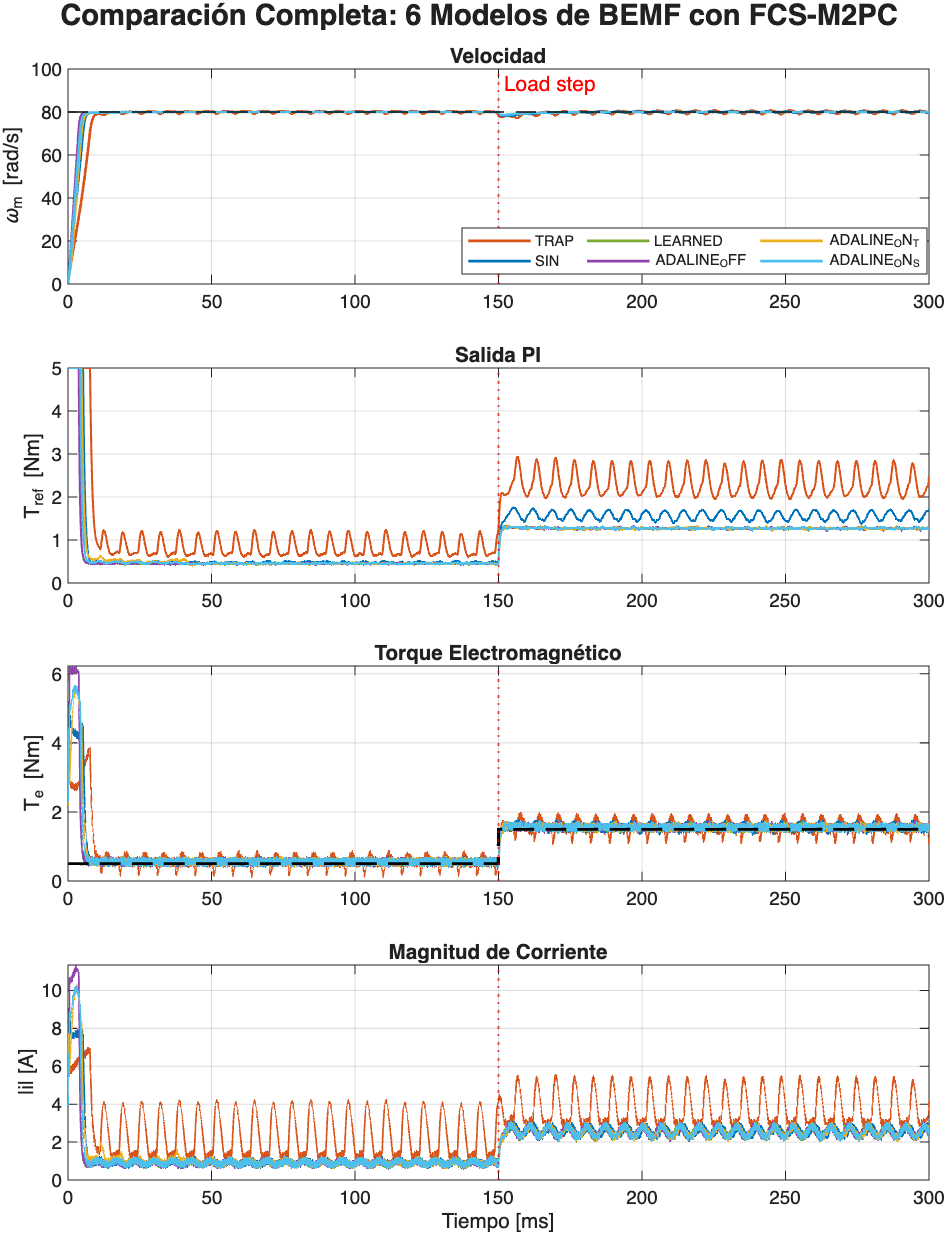
\includegraphics[width=0.35\linewidth]{fig/matlab_panorama.png}\\
        {\footnotesize FCS-M2PC con 6 BEMF y vs Load step}
      \end{center}
\end{frame}

% --- Slide 17: Figuras de simulación ---
\begin{frame}{Respuesta Temporal: Torque y Velocidad}
        \begin{center}
        \centering
        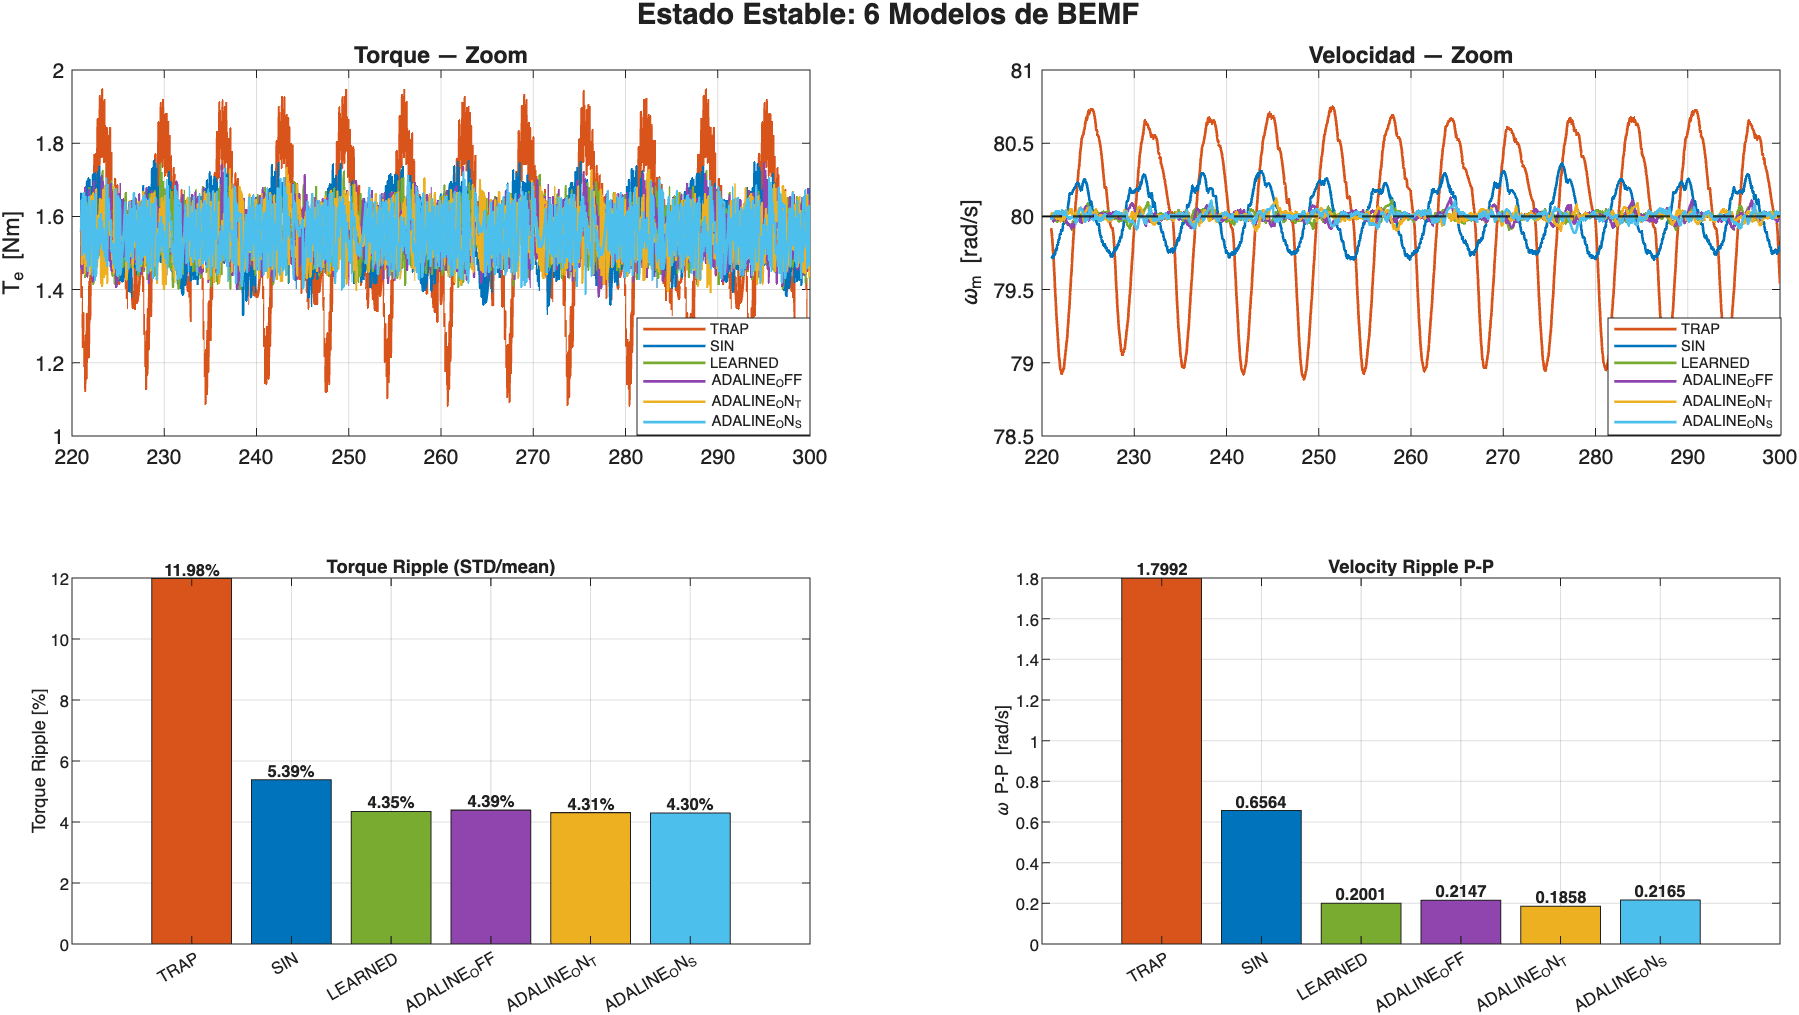
\includegraphics[width=0.75\linewidth]{fig/matlab_zoom_bars.png}\\
        {\footnotesize Zoom SS y Barras ripple}
        \end{center}
        

\end{frame}

% --- Slide 18: Convergencia ---
\begin{frame}{Convergencia del ADALINE Online}
    \begin{center}
        \centering
        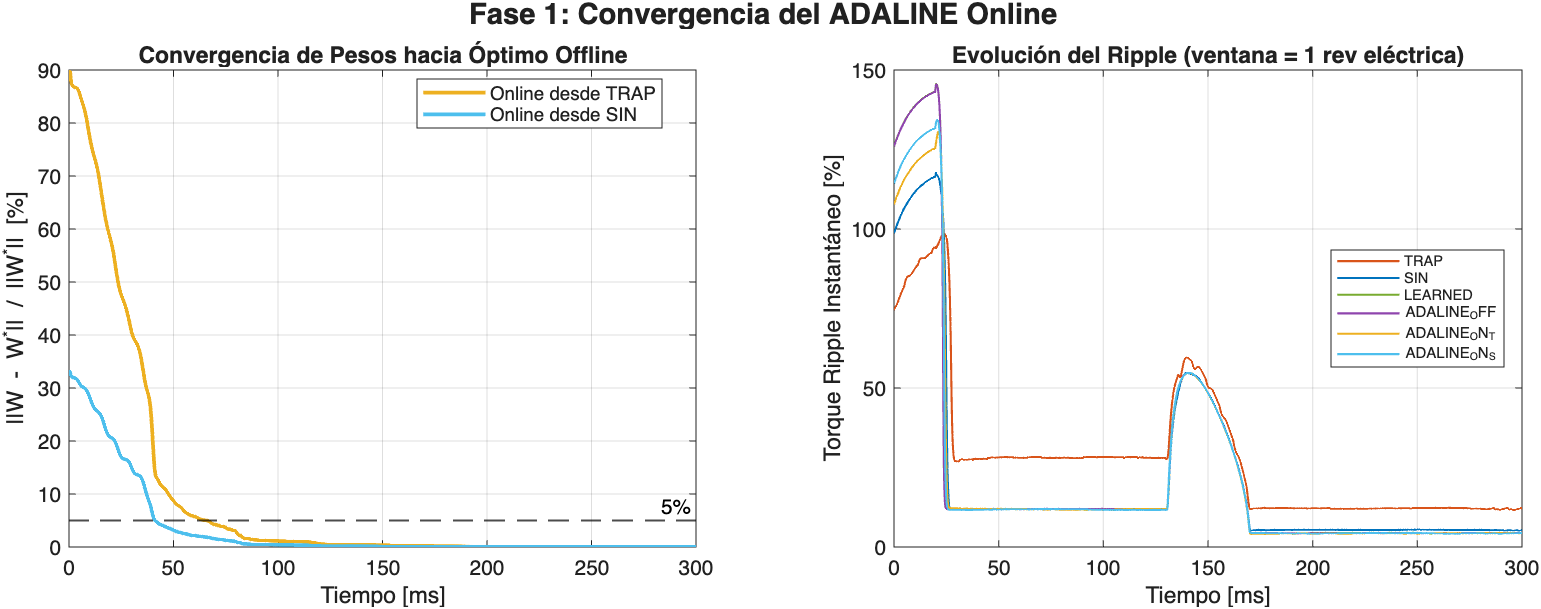
\includegraphics[width=0.95\linewidth]{fig/convergence_matlab.png}
        {\footnotesize Coeficientes de fourier por armónico}
      \end{center}
\end{frame}